% первая часть
\section{Методы получения трехмерных изображений из двумерных}

В ходе выполнения проекта, главным образом, решается задача преобразования двумерных изображений в трехмерные на мобильных устройствах.

В последние годы заметное место в области преобразования и фильтрации изображений занимает задача преобразования двумерных изображений в трехмерные. На сегодняшний день в мире для этого разработаны различные методики, которые позволяют автоматически создавать так называемые «карты глубины»~\cite{depthMap3} (рисунок ~\ref{fig:s-63}) для двумерных изображений, основываясь на свойствах этого изображение и на некоторых предположениях о характере сцены. 

\begin{figure}[H]
	\centering
	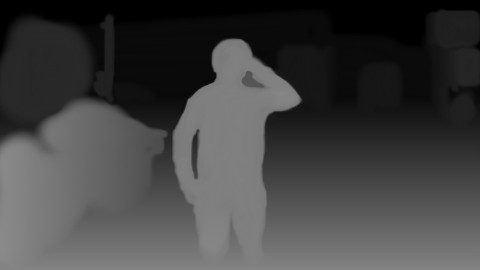
\includegraphics[width=0.7\linewidth]{pics/s-63}
	\caption{карта глубины}
	\label{fig:s-63}
\end{figure} В частности, были проведены исследования следующих методов получения трехмерных изображений из двумерных:

\begin{itemize}
	\item Предположение о том, что изображение имеет линейную перспективу;
	\item Предположение о том, что снимок сделан на открытом пространстве и использование модели рассеяния световых лучей в атмосфере;
	\item Обнаружение теней и восстановление по ним карты глубины;
	\item Обнаружение перекрытий объектов на изображении и используя эту информацию восстановлении карты глубины;
	\item Использование моделей пространственных искажений заданных текстур;
	\item Использование билатеральных симметричных шаблонов;
	\item Использование статистических методов для обучения текстурных шаблонов, на различных расстояниях от объектива и другие методы.
\end{itemize}

Практически все эти методы характеризуются достаточно узким характером сцен, которые могут быть реализованы для преобразования в трехмерное изображение. 

Проведенные предварительные исследования показали, что одним из наиболее перспективных методов преобразования изображений в трехмерные считается метод «дефокусировки», который предполагает, что близкие объекты находятся в фокусе, а более удаленные объекты имеют большее размытие. Используя информацию о размытии той или иной точки на изображении можно предположить о том, насколько далеко она находится от объектива. Используя метод дефокусировки можно построить карту глубины для любой макрофотографии. 

Известные методы получения карты глубины, использующие дефокус удаленных от объектива объектов, основаны на следующей цепочке преобразования изображения~\cite{depthMap1}:

\begin{enumerate} 
	\item Обнаружение краев объектов с использованием фильтра Канни.
	\item Для каждой точки найденного края выполняется оценка расстояния, до нее с использованием гауссовского размытия. Таким образом строится так называемая разреженная карта глубины, которая несет информацию о расстоянии до объектива в некоторых точках изображения. 
	\item Разреженная карта глубины с использованием интерполяции превращается в так называемую «плотную карту глубины», которая уже пригодна для построения трехмерного изображения сцены с любого ракурса. 
\end{enumerate}

Реализация мобильного приложения позволяющего оперативно переводить стандартные фотоизображения в 3D-снимки чрезвычайно актуально и востребовано. С другой стороны, на сегодняшний день имеется определенный научный задел по разработке алгоритмов преобразования 2D -3D. В частности известен ряд различных методик, которые позволяют автоматически создавать «карты глубины» для двумерных изображений, основываясь на свойствах этого изображение, и на некоторых предположениях о характере сцены. Например метод дефокусировки позволяет построить карту глубины фотографии. Вместе с тем информации о программно реализованных в том числе мобильных приложений крайне мало. 

Рассмотренный метод преобразования (см. пункты 1-3) предыдущего раздела страдает двумя существенными недостатками\cite{depthMap2}.

\begin{enumerate}
	\item Разреженная карта глубины получается не всегда гладкой, что приводит к ошибкам последующей интерполяции и, в итоге, к ошибкам в карте глубины. 
	\item Окончательная интерполяция для построения требует больших вычислительных затрат и до последнего времени не имела возможности быть встроенной в мобильные приложения. 
\end{enumerate}

Основываясь на этих двух недостатках существующего метода дефокусировки изображения, требуется провести научное исследование в следующих направлениях:

\begin{enumerate}
	\item Адаптивное сглаживание разреженной карты глубины.  С использованием методов кластеризации краев изображения, в протяженные структуры, глубина точек которых должна подчиняться некоторому закону, а не быть случайной от точки к точке, как в существующем методе. 
	\item Найти способ снижения вычислительных затрат для выполнения двумерной интерполяции при построении плотной карты глубины. 
	\item Нам представляется, что для преобразования двумерного видеоролика в трехмерное представление необходимо разработать методику передачи разреженной карты глубины (с учетом сглаживания) от кадра к кадру. 
\end{enumerate}

Таким образом предлагаемый Проект на сегодняшний день актуален и содержит помимо научной алгоритмической составляющей широкие перспективы коммерциализации.

\subsection{Восстановление глубины из одного расфокусированного изображения}

Рассмотрим сложную задачу восстановления глубины из одного расфокусированного изображения. Входное расфокусированное изображение повторно размыто с использованием гауссова ядра, а значение размытости размытия может быть получено из коэффициента градиента между входными и повторно размытыми изображениями. Распространяя количество размытия в крайних положениях на все изображение, можно восстановить всю карту глубины сцены.

Результат восстановления глубины нашего метода. (рисунок~\ref{fig:input}) Большая интенсивность означает большую глубину на всех картах глубины

\begin{figure}[H]
	\centering
	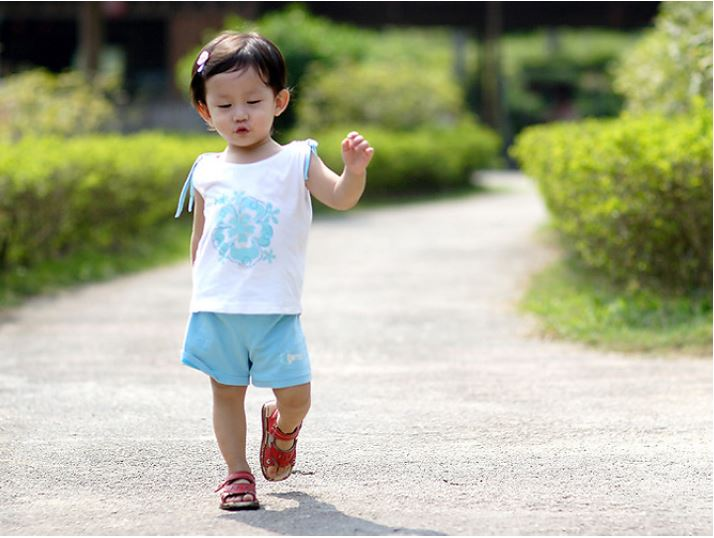
\includegraphics[width=0.4\linewidth]{pics/input}
	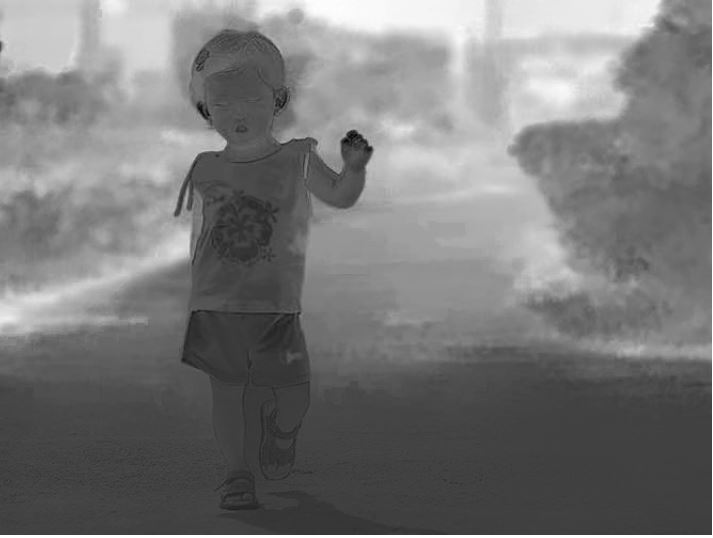
\includegraphics[width=0.4\linewidth]{pics/depth_map}
	\caption{Входное изображение и карта глубины}
	\label{fig:input}
\end{figure}

Сосредоточимся на более сложной проблеме восстановления относительной глубины из одного расфокусированного изображения, захваченного некалиброванной обычной камерой. Метод обратной диффузии~\cite{Proc} моделирует размытие дефокусировки в качестве процесса диффузии тепла и использует неоднородную диффузию тепла для оценки размытости размытия в краевых положениях. В отличие от этого, моделируем размытие дефокусировки как размытие 2D Gaussian. Входное изображение повторно размывается с использованием известного гауссовского размытия, и рассчитывается коэффициент градиента между входными и повторно размытыми изображениями. Величина размытия в краевых местоположениях может быть получена из отношения.

Рассмотрим эффективный метод оценки размытия, основанный на гауссовском градиентном соотношении, и показываем, что он устойчив к шуму, неточному расположению краев и помехам от соседних ребер. Без каких-либо изменений в камерах или при использовании дополнительного освещения наш метод позволяет получить карту глубины сцены, используя только одно расфокусированное изображение, снятое обычной камерой. Как показано (рисунок~\ref{fig:input}), этот метод может извлекать карту глубины сцены с довольно высокой степенью точности.

\subsection{Модель дефокусировки}

Оцениваем размытие размытия в местах краев и предполагаем, что края являются ступенчатыми краями. Идеальный край шага может быть смоделирован как:

\begin{equation}\label{eq:1}
f(x)=Au(x)+B
\end{equation}

где $u(x)$ - ступенчатая функция. A и B - амплитуда и смещение края соответственно. Обратите внимание, что ребро расположено в точке $x=0$.

Предположим, что фокус и дефокусировка подчиняются тонкой модели объектива~\cite{Optics}. Когда объект размещается на расстоянии фокусировки $d_f$, все лучи от точки объекта будут сходиться к одной точке датчика, и изображение будет резким. Лучи из точки другого объекта на расстоянии $d$ достигают нескольких точек датчика и приводят к размытому изображению. Размытый рисунок зависит от формы апертуры и называется кругом путаницы (CoC)~\cite{Optics}. Диаметр CoC характеризует величину расфокусировки и может быть записан как

\begin{equation}\label{eq:2}
c=\frac{|d-d_f|}{d}\frac{f_0^2}{N(d_f-f_0)}
\end{equation}

\begin{figure}[H]
	\centering
	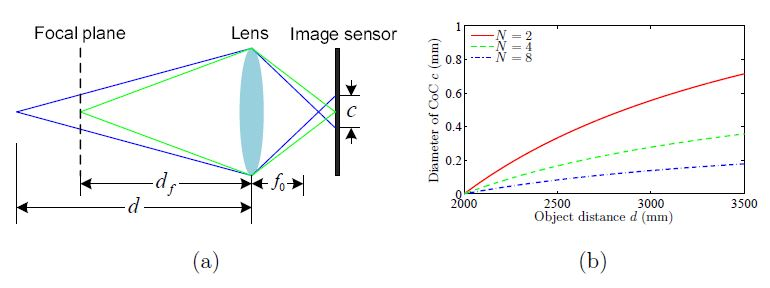
\includegraphics[width=1\linewidth]{pics/focus}
	\caption{Тонкая модель объектива}
	\label{fig:focus}
\end{figure}

где $f_0$ и $N$ - фокусное расстояние и номер остановки камеры соответственно. На рисунке~\ref{fig:focus} показаны фокус и расфокусировка для модели тонких линз и как изменяется диаметр круга замешательства с $d$ и $N$, при фиксированном $f_0$ и $d_f$.
Как мы видим, диаметр CoC $c$ является нелинейной монотонно возрастающей функцией расстояния объекта $d$. Размытие дефокусировки может быть смоделировано как свертка острого изображения с функцией распределения точек (PSF). PSF обычно аппроксимируется гауссовой функцией $g(x,\sigma)$, где стандартное отклонение $\sigma=kc$ пропорционально диаметру CoC $c$. Используем $\sigma$ как меру глубины сцены. Следовательно, размытие ребра $i(x)$ можно представить следующим образом,

\begin{equation}\label{eq:3}
i(x)=f(x)\otimes g(x,\sigma)
\end{equation}

\subsection{Оценка размытости}

На рисунке~\ref{fig:blur} показан обзор метода оценки размытия. Граница шага повторно размыта с использованием гауссова ядра с известным стандартным отклонением. затем рассчитывается соотношение между величиной градиента края ступени и ее размытой версией. Это максимальное значение в краевом положении. Используя максимальное значение, можем вычислить величину размытости дефокусировки в местоположении края.

\begin{figure}[H]
	\centering
	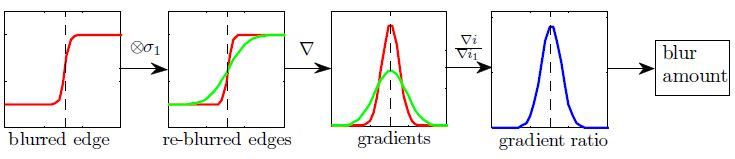
\includegraphics[width=1\linewidth]{pics/blur}
	\caption{Оценка размытости, черная штриховая линия обозначает местоположение края}
	\label{fig:blur}
\end{figure}

Используем двумерное изотропное гауссовское ядро для повторного размытия и величину градиента можно вычислить следующим образом:

\begin{equation}\label{eq:4}
||\bigtriangledown i(x,y)||=\sqrt{\bigtriangledown i_x^2+\bigtriangledown i_y^2}
\end{equation}

где $\bigtriangledown i_x$ и $\bigtriangledown i_y$- градиенты вдоль направлений x и y соответственно. Устанавливаем повторное размытие $\sigma_0=1$ и используем детектор края Canny ~\cite{IEEE} для выполнения обнаружения края.
Шкала размытия оценивается в каждом краевом положении, образуя редкую
карта глубины, обозначаемая $\hat{d}(x)$. Однако из-за шума или мягких теней оценки размытия могут содержать некоторые ошибки. Чтобы подавить эти ошибки, применяется совместный двусторонний фильтр ~\cite{ACM} на разреженной карте глубин $\hat{d}(x)$. Выход совместного двустороннего фильтра в каждом краевом положении х определяется как:

\begin{equation}\label{eq:5}
BF(\hat{d}(x))=\frac{1}{W(x)}\sum_{y\in N(x)}G_{\sigma s}(||x-y||)G_{\sigma r}(||I(x)-I(j)||)\hat{d}(y)
\end{equation}

где $W(x)$ - коэффициент нормировки, а $N(x)$ - окрестность точки x, заданная размером пространственного гауссовского фильтра $G_{\sigma s}$. Фильтрация выполняется только по краям. Совместный двусторонний фильтр корректирует некоторые ошибки в разреженной карте глубины и избегать распространения этих ошибок в интерполяции глубины, описанной в следующем разделе.


\subsection{Интерполяция глубины}

Данный метод оценки размытия дает разреженную карту глубин $d(x)$ с оценками глубины в местах краев. Чтобы получить полную карту глубины $d(x)$, необходимо распространить эти значения из местоположений краев на все изображение. Найдем регуляризованное отображение глубины $d(x)$, которое близко к разреженной карте глубин $d(x)$ в каждом краевом положении. Для этих задач обычно используются методы интерполяции с учетом края~\cite{ACM2}. Здесь применяется матирующий лапласиан~\cite{IEEE2} для выполнения интерполяции.
Мы переписываем разреженную карту глубин d (x) и полное отображение глубины d (x) в их векторной форме как d и d. Тогда проблему интерполяции глубины можно сформулировать как минимизирующую следующую функцию стоимости:


\subsection{Тестирование стабильности и качества алгоритма}

\begin{figure}[H]
	\centering
	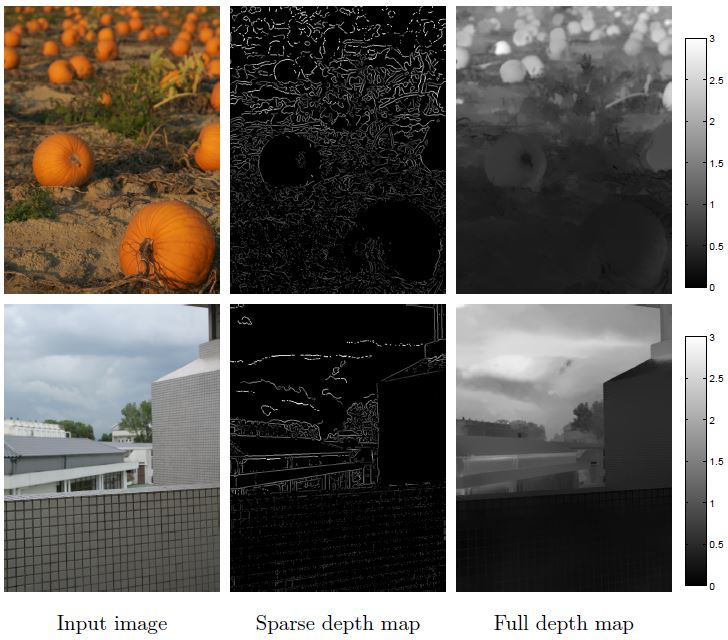
\includegraphics[width=0.7\linewidth]{pics/comparison}
	\caption{Восстановление глубины на реальных изображениях. Наш метод может работать как на сценах с непрерывной глубиной (изображение тыквы), так и на слоистой глубине (изображение здания) для получения карты глубины с довольно хорошей точностью.}
	\label{fig:comparison}
\end{figure}\

Как показано на рисунке~\ref{fig:comparison}, я тестирую наш метод на некоторых реальных изображениях. В изображении тыквы глубина сцены непрерывно изменяется от нижней к верхней части изображения. Оценочная карта глубины фиксирует непрерывное изменение глубины. В изображении здания сцена в основном содержит три слоя: стены, дом и небо. Наш метод позволяет создавать карты глубин, точно представляющие эти слои глубины. Как видно из результатов, наш метод позволяет точно восстановить глубину сцены из одного расфокусированного изображения. На рисунке~\ref{fig:flower} мы сравниваем наш метод с методом обратной диффузии~\cite{Proc}.

\begin{figure}[H]
	\centering
	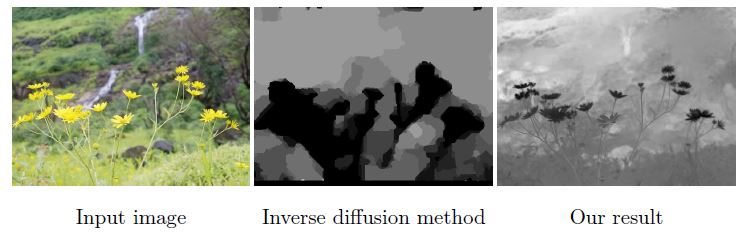
\includegraphics[width=1\linewidth]{pics/flower}
	\caption{Сравнение нашего метода с методом обратной диффузии, на примере цветка}
	\label{fig:flower}
\end{figure}\

Метод обратной диффузии создает грубую слоистую карту глубины. В результате этого цветочный слой плохо отделен фоновыми слоями и содержит некоторые оценки погрешности. Напротив, наш метод способен производить более точную и непрерывную карту глубины, а цветочный слой хорошо отделен фоновой травой и деревьями.

\subsection{Оценка достоверности построения карты глубины}

В ходе выполнения проекта будет создана методика количественной оценки достоверности построения карты глубины, которая необходима для корректного преобразования 2D изображения в 3D вид. Эта методика основана на сравнении показаний глубины, полученных в результате работы алгоритмов преобразования 2D –> 3D и достоверных показаний глубины для данной сцены, которые получены в ручном режиме.

Для реализации методики предполагается произвести ручную разметку тестовых цифровых фотографий в количестве не менее 100 штук. Для этого в ручном режиме устанавливаются контрольные точки, с указанием расстояния до них.

Таким образом формируется разреженная карта глубины, с указанием абсолютных значений. Далее, на изображении находится самая дальняя контрольная точка и все расстояния нормируются на расстояние до нее. Таким образом формируется разреженная карта глубины с относительными расстояниями, и, как следствие, (алгоритмически) формируется «эталонная» плотная карта глубины.

Далее, в результате работы различных алгоритмов преобразования изображения из двумерного в трехмерное автоматически вычисляется как разреженная карта глубины для каждого из анализируемых алгоритмов (создаваемого в рамках проекта и конкурирующих аналогов). Далее предполагается вычислять среднеквадратичную ошибку между эталонными значениями для карты глубины и значениями, вычисленными каждым из алгоритмов.

Предполагается, что алгоритм, реализуемый в ходе выполнения проекта даст снижение такой ошибки между вычисленными и эталонными значениями на величину не менее 25\% (ожидаемое значение – порядка 30\%).

\section{Описание предметной области}
В ходе выполнения проекта, главным образом, решается задача преобразования двумерных изображений в трехмерные(GIF) на мобильных устройствах.

В последние годы заметное место в области преобразования и фильтрации изображений занимает задача преобразования двумерных изображений в трехмерные. На сегодняшний день в мире для этого разработаны различные методики, которые позволяют автоматически создавать так называемые «карты глубины» для двумерных изображений, основываясь на свойствах этого изображение и на некоторых предположениях о характере сцены. 

\subsection{Android Studio}
Android Studio - полностью укомплектованная платформа для разработки и тестирования приложений под операционную систему Android. Разработчики этой оболочки (компания Google) внедрили весь необходимый инструментарий для удобного и качественного проектирования новых приложений и доработки существующих. Программа включает в себя такие компоненты как Android SDK, все версии операционки Android, эмулятор для запуска приложений, элементы тестирования и отладки программ.

Создавая новый проект, будет доступна полная структура приложения со всеми файлами, что позволяет более четко и продуманно организовать сам процесс разработки. Очень удобно реализован показ вносимых изменений и дополнений - визуально в реальном времени происходят преобразования в зависимости от заданных действий. Что немаловажно, программа позволяет делать разработку приложений для всех версий ОС Andriod и для различных устройств - можно предварительно оценить внешний вид программы, например, под планшет или смартфон.

Среда Android Studio предназначена как для небольших команд разработчиков мобильных приложений (даже в количестве одного человека), или же крупных международных организаций с GIT или другими подобными системами управления версиями. Опытные разработчики смогут выбрать инструменты, которые больше подходят для масштабных проектов. Решения для Android разрабатываются в Android Studio с использованием Java или C++. В основе рабочего процесса Android Studio заложен концепт непрерывной интеграции, позволяющий сразу же обнаруживать имеющиеся проблемы. Продолжительная проверка кода обеспечивает возможность эффективной обратной связи с разработчиками. Такая опция позволяет быстрее опубликовать версию мобильного приложения в Google Play App Store. В Android Studio есть удобная маркировка кода, которая позволит без труда ориентироваться в больших проектах. Кроме того, отдельные компоненты можно изменять простым перетаскиванием в другое нужное место, что значительно упрощает редактирование.

\subsection{Java}
Преимущества языка Java
\begin{itemize}
	\item Одно из основных преимуществ языка Java — независимость от платформы, на которой выполняются программы: один и тот же код можно запускать под управлением операционных систем Windows, Solaris, Linux, Machintosh и др. 
	Это действительно необходимо, когда программы загружаются через Интернет для последующего выполнения под управлением разных операционных систем.
	\item Другое преимущество заключается в том, что синтаксис языка Java похож на синтаксис языка C++, и программистам, знающим языки С и C++, его изучение не составляет труда.
	\item Кроме того, Java — полностью объектно-ориентированный язык, даже в большей степени, чем C++. Все сущности в языке Java являются объектами, за исключением немногих основных типов (primitive types), например чисел.
	\item Исключена возможность явного выделения и освобождения памяти.	Память в языке Java освобождается автоматически с помощью механизма сборки мусора. Программист гарантирован от ошибок, связанных с неправильным использованием памяти.
	\item Безопасный: методы проверки подлинности основаны на шифровании с открытым ключом.
	\item Динамический: программирование на Java считается более динамичным, чем на C или C++, так как он предназначен для адаптации к меняющимся условиям. Программы могут выполнять обширное количество во время обработки информации, которая может быть использована для проверки и разрешения доступа к объектам на время выполнения.
\end{itemize}

\subsection{Технические требования.}

Необходимая задача при реализации проекта - адаптация существующего метода преобразования 2D в 3D для использования под управлением операционной системы Android.

В ходе выполнения проекта будут созданы мобильные приложения со следующими характеристиками:

\begin{itemize}
	\item мобильное приложение, функционирующее под управлением операционной системы Android версии не ниже 5.0.
	\item специальных дополнительных требований к аппаратному обеспечению мобильных устройств не предъявляется. Они соответствуют требованиям, накладываемым вышеперечисленными версиями ОС.
	\item мобильные приложения должны функционировать на устройствах с разными размерами экрана от 2.6 до 6 дюймов с разрешениями от 240х320 до 1440х2560 пикселей.
	\item источник данных для конвертирования - файлы в формате jpeg из галереи мобильного устройства или фотография, сделанная штатной фотокамерой мобильного устройства.
	\item мобильные приложения должны обеспечивать конвертацию сделанных фотокамерой изображений при максимальном качестве съемки не менее 10 Мп.
	\item формат данных, в которых сохраняются результаты --- анаглиф файлы (формат jpeg), стерео пара (формат jps), анимированные файлы в формате gif.
	\item ориентировочное время преобразования 2D в 3D не должно превышать 5 секунд.
\end{itemize}

\subsection{Изучение основ разработки мобильного приложения в среде Android Studio}

Android основан на Linux. Между приложением и ядром лежит слой API и слой библиотек на нативном коде. Приложение выполняется на виртуальной машине Java (Dalvik Virtual Machine).
В Android можно запускать много приложений. Но одно из них есть главным и занимает экран. От текущего приложения можно перейти к предыдущему или запустить новое. Это похоже на браузер с историей просмотров.

Каждый экран пользовательского интерфейса представлен классом Activity в коде. Различные Activity содержатся в процессах. Activity может даже жить дольше процесса. Activity может быть приостановлена и запущена вновь с сохранением всей нужной информации.(рисунок~\ref{fig:activity})

\begin{figure}[H]
	\centering
	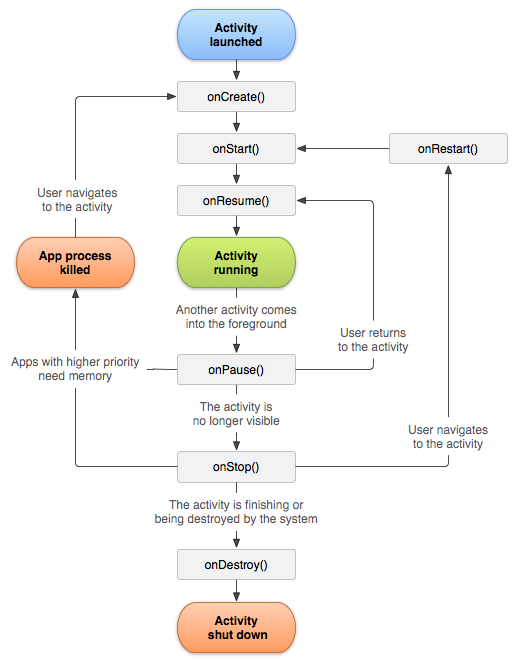
\includegraphics[width=0.6\linewidth]{pics/activity}
	\caption{activity}
	\label{fig:activity}
\end{figure}

Android использует специальный механизм описания действий основанный на Intent. Когда нужно выполнить действие (сделать звонок, послать письмо, показать окно), вызывается Intent.

Также Android содержит сервисы подобные демонам в Linux для выполнения нужных действий в фоновом режиме (например, проигрывание музыки).
Для обмена данными между приложениями используются Content providers (провайдеры содержимого).

Содержимое Activity формируется из различных компонентов, называемых View. Самые распространенные View - это кнопка, поле ввода, чекбокс и т.д. (рисунок~\ref{fig:view})

\begin{figure}[H]
	\centering
	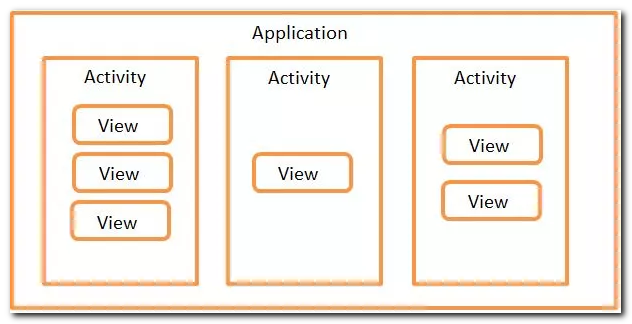
\includegraphics[width=0.6\linewidth]{pics/view}
	\caption{view}
	\label{fig:view}
\end{figure}

Необходимо заметить, что View обычно размещаются в ViewGroup. Самый распространенный пример ViewGroup – это Layout. Layout бывает различных типов и отвечает за то, как будут расположены его дочерние View на экране.

LinearLayout – отображает View-элементы в виде одной строки (если он Horizontal) или одного столбца (если он Vertical).

TableLayout – отображает элементы в виде таблицы, по строкам и столбцам.

RelativeLayout – для каждого элемента настраивается его положение относительно других элементов.

AbsoluteLayout – для каждого элемента указывается явная позиция на экране в системе координат (x,y)

\subsection{Основные компоненты пользовательского интерфейса мобильного приложения в Android}

В Android используется UI-фреймворк, сравнимый с другими полнофункциональными UI-фреймворками, применяемыми на локальных компьютерах. Он является более современным и асинхронным по природе. По существу, UI-фреймворк Android относится уже к четвертому поколению, если считать первым поколением традиционный прикладной интерфейс программирования Microsoft Windows, основанный на С, а MFC (Microsoft Foundation Classes, библиотека базовых классов Microsoft на основе C++) - вторым. В таком случае UI-фреймворк Swing, основанный на Java, будет третьим поколением, так как предлагаемые в нем возможности дизайна значительно превосходят по гибкости MFC. Android UI, JavaFX, Microsoft Silverlight и язык пользовательских интерфейсов Mozilla XML (XUL) относятся к новому типу UI-фреймворков четвертого поколения, в котором UI является декларативным и поддерживает независимую темизацию.

При программировании в пользовательском интерфейсе Android применяется объявление интерфейса в файлах XML. Затем эти определения представления (view definitions) XML загружаются в приложение с пользовательским интерфейсом как окна. Даже меню приложения загружаются из файлов XML. Экраны (окна) Android часто называются активностями (activities), которые включают в себя несколько видов, нужных пользователю, чтобы выполнить логический элемент процесса. Виды (views) являются основными элементами, из которых в Android состоит пользовательский интерфейс. Виды можно объединять в группы (view groups). Для внутренней организации видов используются давно известные в программировании концепции холст (canvas), рисование (painting) и взаимодействие пользователя с системой (user interaction).

Такие составные представления, в которые входят виды и группы видов, работают на базе специального логического заменяемого компонента пользовательского интерфейса Android.

Одной из ключевых концепций фреймворка Android является управление жизненным циклом (lifecycle) окон явлений (activity windows). В системе применяются протоколы, поэтому Android может управлять ситуацией по мере того, как пользователи скрывают, восстанавливают, останавливают и закрывают окна явлений.


\section{Разработка концепции и архитектуры мобильных приложений, предназначенных для преобразования 2D в 3D.}
В ходе выполнения работы были рассмотрены различные варианты для создания мобильных приложений, предназначенных для преобразования 2D изображений в 3D вид. При этом рассмотрении учитывалось, что результирующие мобильные приложения должны создаваться под операционные системы Android и iOS, а также то, что один из основных результатов работы приложения с точки зрения конечного пользователя – это возможность публикации созданного 3D-изображения в виде анимированного gif-файла в одном или нескольких аккаунтов в социальных сетях пользователя. Соответственно, можно исходить из предположения о том, что для функционирования приложения в любом случае необходим доступ к сети интернет. Максимальная унификация различных составных частей приложения между собой хотя бы на уровне исходных кодов вне зависимости от целевой платформы (Android или iOS) является дополнительным преимуществом при рассмотрении различных вариантов создания мобильных приложений.

Один из наиболее простых с технической точки зрения вариантов реализации решения, позволяющего преобразовывать 2D файлы в 3D вид, является решение, основанное на создании веб-сервиса, который предоставляет минимально необходимый пользовательский интерфейс для загрузки желаемого файла на сервер, преобразования файла на сервере и, как результат, возможность скачать получившийся файл на устройство пользователя и поделиться этим файлом в социальных сетях. При простоте архитектуры у этого решения есть один существенных недостаток – как правило, такие решения менее удобны и функциональны, чем нативные (native) мобильные приложения, разработанные специально под целевую платформу, на которой они будут функционировать. Поэтому на данном этапе от такого подхода было принято решение отказаться.

Если рассматривать варианты создания нативных мобильных приложений, существует несколько возможных вариантов:

\begin{enumerate}
	\item Использовать наиболее популярные средства разработки и языки программирования для каждой из необходимых мобильных платформ. Создать нативное мобильное приложение, реализующее весь необходимый пользовательский интерфейс, набор сервисных функций. Портировать алгоритм преобразования графического файла из 2D в 3D для локального исполнения на мобильном устройстве. Все необходимые преобразования выполнять локально, на мобильном устройстве. Полученный результат преобразования (анимированный gif) загружать в интернет (социальные сети) по мере его готовности на мобильном устройстве.
	\item Использовать наиболее популярные средства разработки и языки программирования для каждой из необходимых мобильных платформ для создания нативных мобильных приложений только для реализации пользовательского интерфейса и набора сервисных функций. Алгоритм преобразования графического файла из 2D в 3D реализуется в виде серверного модуля, соответственно для преобразования выбранного файла и предварительного просмотра полученных результатов необходимо загрузить этот выбранный файл на сервер. Загрузить полученный результат с сервера и поделиться этим результатом в социальных сетях.
	\item Использовать кроссплатформенное средство разработки мобильных решений Xamarin. Это средство одновременно позволяет создавать iOS, Android и Windows Phone приложения. Реализация алгоритма преобразования графического файла из 2D в 3D модифицируется таким образом, что может быть непосредственно интегрирована в Xamarin-проект. В результате получается единое решение, которое на этапе сборки может быть превращено в полнофункциональное нативное приложение для любой из поддерживаемых платформ --- iOS, Android и Windows Phone. Результирующее решение будет преобразовывать графические файлы из 2D в 3D локально на мобильном устройстве, доступ к интернету необходим только для реализации функции «поделиться созданным 3D-файлом в социальных сетях».
	\item Использовать кроссплатформенное средство разработки мобильных решений Xamarin, но только лишь для создания нативных мобильных приложений. реализующих пользовательский интерфейс и набор сервисных функций. Алгоритм преобразования графического файла из 2D в 3D реализуется в виде серверного модуля, соответственно для преобразования выбранного файла и предварительного просмотра полученных результатов необходимо загрузить этот выбранный файл на сервер. Загрузить полученный результат с сервера и поделиться этим результатом в социальных сетях.
\end{enumerate}

Перед тем, как рассмотреть каждый из приведенных выше вариантов по отдельности, следует отметить, что существующая на сегодняшний день реализация алгоритма преобразования изображений из 2D в 3D вид реализована на языке С++, сборка осуществляется с использованием Microsoft Visual Studio, соответствующее решение имеет существенную зависимость от OpenCV (Open Source Computer Vision Library – это программная библиотека с открытым исходным кодом, реализующая базовые алгоритмы компьютерного зрения, обработки изображений и численных алгоритмов общего назначения. Реализована на C/C++).

Возвращаемся к вышеперечисленным вариантам.

Для варианта №1 для операционной системы Android необходимо:

С использованием Android Studio на языке программирования Java реализовать необходимый пользовательский интерфейс, а также весь необходимый набор сервисных функций. Необходимо адаптировать реализацию алгоритма преобразования графического файла из 2D в 3D для использования под управлением операционной системы Android (реализация на С++). Далее, с использованием механизма The Android Native Development Kit (NDK) необходимо обеспечить вызов кода, написанного на языке С++ из «классического» Android-приложения. 

Для разработки приложений для iOS основным средством разработки является Objective-C. Проведенные предварительные исследования показали, что адаптировать реализацию алгоритма преобразования графического файла из 2D в 3D для использования под управлением операционной системы iOS с разумными усилиями не представляется возможным. Соответственно, вариант №1 является неприемлемым для реализации решения для операционной системы iOS.

Для реализации варианта №2 необходимо:

С использованием наиболее популярных средств разработки и языков программирования для каждой из необходимых мобильных платформ (Java для Android и Objective С для iOS) необходимо создать нативные мобильных приложений для реализации пользовательского интерфейса и набора сервисных функций. Эта задача, в целом, является типовой и принципиальных сложностей не вызывает. Алгоритм преобразования графического файла из 2D в 3D следует реализовать в виде серверного модуля, например, для использования под управлением операционной системы Ubuntu. Это обусловлено тем, что Unix-подобные операционные системы имеют существенно более широкое распространение в Web-серверном окружении, чем Windows-сервера. Основная сложность данной задачи – в сборке и корректном использовании OpenCV библиотеки под Linux, однако аналогичная задача сравнительно недавно была решена коллегами для реализации демонстрационного видеоплеера для использования под операционной системой Ubuntu.

Для реализации варианта №3 необходимо адаптировать алгоритм преобразования графического файла из 2D в 3D таким образом, чтобы он мог быть непосредственно интегрирован в Xamarin-проект (разработка на языке программирования С\#). Проведенные предварительные исследования показали, что реализовать подобный функционал за разумное время с разумными усилиями не представляется возможным.

Вариант №4 основывается на разработке унифицированного решения для всех поддерживаемых мобильных платформ (iOS, Android и Windows Phone) для реализации пользовательского интерфейса и сервисных функций на языке программирования С\#. В части алгоритма преобразования графического файла из 2D в 3D этот вариант полностью аналогичен (точнее даже унифицирован) варианту №2 – должен быть реализован серверный модуль, например, для использования под управлением операционной системы Ubuntu для реализации этого преобразования. И, соответственно, с помощью реализованных на С\# функций выбирается файл для преобразования, отправляется на сервер, там преобразовывается, скачивается обратно для предварительного просмотра полученных результатов, а далее реализуется возможность поделиться полученным результатом в социальных сетях.

На основе проведенного исследования можно сделать следующий вывод. С точки зрения скорости, легкости и качества реализации наиболее перспективными являются варианты №2 и №4. Однако, вариант №4, в силу кроссплатформенности, унифицированности решения для всех поддерживаемых мобильных платформ является более предпочтительным. Соответственно, на реализации этого варианта и будут сосредоточены усилия на самом первом этапе развития проекта. 

Очевидным недостатком подобного решения является существенная его зависимость от скорости и надежности мобильного интернета, а также от доступности конечному пользователю оплаченного траффика. Для обхода этих ограничений предполагается исследовать возможность создания для пользователей ОС Android «самодостаточного» мобильного приложения (вариант №1), которое все необходимые действия, связанные с преобразованием файлов производит непосредственно на мобильном устройстве. Хочется надеяться, что необходимая для этого адаптация алгоритма преобразования графического файла из 2D в 3D для использования под управлением операционной системы Android (после создания реализации этого алгоритма по Ubuntu, основная проблема – возможность использования OpenCV под соответствующую платформу – должна решаться аналогичным образом) не доставит много хлопот.
